\hypertarget{paper-3}{%
\chapter{Social Norms under Uncertain Times: A dynamic study of Stay-At-Home and Vaccination Rates During the Covid-19 Pandemic}\label{paper-3}}

\hypertarget{abstract-1}{%
\section{Abstract}\label{abstract-1}}

This paper examines how social norms are formed under conditions of uncertainty
using the case studies of stay-at-home and vaccination rates during the Covid-19
pandemic. I test fear-based models of behavioral adaption to public health
recommendations as well as patterns of complex social contagion using linear
mixed effects models. These models show that complex contagion is a valid
framework for the social contagion of new norms during Covid-19. However, I find
important moderating effect of signal discordance, the contextual diversity of
signals received by an ego.

% need to explain a little bit more what diversity of signals etc means (since this is the first look) 
% what else needs to be said here to properly convey the importance and impact of this finding? 

Keywords: Social Networks, Social Norms, Health Behavior, Diffusion, Contagion

% TODO
\citep{mirbabaie_etal20, ternullo22}

\hypertarget{background}{%
\section{Background}\label{background}}

After spreading around the world in a matter of months, the coronavirus
(COVID-19) became a leading cause of death in the United States. Although the
Centers for Disease Control and Prevention (CDC) \citeyearpar{centersfordiseasecontrolandpreventionHowProtectYourself2020} proposed several potential mitigation strategies, the method of mitigation that received the most national
attention is the call to stay-at-home and social distance for non-essential
workers. CDC officials and frontline health care professionals advise that the
best way to prevent exposure to the virus is to stay at home and avoid close
contact with people.

A second strategy pushed by the CDC, once available, was to receive vaccination
to prevent the effects of the Covid-19 virus if infected. Vaccinations like
Pfizer-BioNTech (Comirnaty, tozinameran, BNT162b2), and Janssen/Johnson \&
Johnson, Moderna (mRNA-1273) started receiving approval for emergency use
authorization by the United States Food and Drug Administration (FDA) in
December 2020.

Although these public health interventions were pushed by policy makers
throughout 2020 and 2021, policy makers often struggle to promote public
adoption of policies that rely on the publics' willingness to adjust their
current `risky' behaviors to less-risk behaviors based on scientific facts. The
lack of adaption to newly recommended behaviors is partially due to the
variation in how individuals came to understand the threats of the disease
\citep{akpanAssociationWhatPeople2021, bailey_etal20}, but also due to habitus: the
ingrained habits, skills and dispositions of individuals and groups
\citep{bourdieu77}. Habitus shapes how individuals perceive different social
interactions and norms and shape how they adopt different policies, leading to
different social outcomes and a divergence of attitudes \citep{scottarthur_etal21, williams95, madeira_etal18}.

There is little research on stay-at-home rates, especially in cases of pandemics
or disasters. Though research on the causes of population mobility did expand
after the onset of the Covid-19 pandemic 
\citep{bargainTrustCompliancePublic2020, bourassaStatelevelStayathomeOrders2020, bourassaSocialDistancingHealth2020, grossmanPoliticalPartisanshipInfluences2020, haggerPredictingSocialDistancing2020, hillBloodChristCompels2020, hillNastiestQuestion, hillLoveThyAged2021,huynhDoesCultureMatter2020}, most research focused on unchanging cultural
determinants of the reduction in stay-at-home rates. For instance, \citet{gibbons_etal21}
 finds that social capital had spatially inconsistent effects on
stay-at-home rates. Instead of focusing on cultural relationships with
stay-at-home rates, this paper will instead focus on the dynamic nature of
population mobility across population networks.

There is more research on vaccine uptake \citep{schmidBarriersInfluenzaVaccination2017}
 because of increased hesitancy and
anti-vaccination movements over previous decades \citep{baumgaertnerInfluencePoliticalIdeology2018, hornseyDonaldTrumpVaccination2020, johnsonOnlineCompetitionPro2020, whiteheadHowCultureWars2020}. While some studies use social network analysis to
study the discussions for an against vaccinations online \citep{milaniVisualVaccineDebate2020}, vaccination rates are a great way to
investigate the establishment of new social norms. First, vaccination uptake is
measurable with stable information tracking infrastructure and vaccination
rates are varied across locations and time. Secondly, because vaccines have 
become politicized \citep{mottaRepublicansNotDemocrats2021, mottaIdentifyingPrevalenceCorrelates2021}, the social contagion effects can be
studied.

This article researches the formation of social norms governing health behaviors
in cases of extreme uncertainty during the Covid-19 pandemic. Using theories of complex
contagion, associative diffusion and the integrated theoretical framework of
norms, I test how these health behaviors are outcomes of contagion and
discordance of signals, as well as other factors affecting associations like
religious and political conservatism, attention to television media sources,
and online norms as measured by information-search behaviors. Before outlining
my central hypotheses, I offer an overview of the current state of the social
contagion literature. After that, I will outline how I compiled this unique
longitudinal data set from Google, the CDC, Facebook and other sources and how I
define and calculate signal and discordance, two key independent variables for
this paper. To model stay-at-home and vaccination rates, I use linear mixed effects
models with random effects as a longitudinal model of contagion. After
interpreting the results of the models, I discuss the implications of these
findings for the sociological understanding of social contagion and the
formation of social norms.

\hypertarget{the-social-contagion-model}{%
\subsection{The Social Contagion Model}\label{the-social-contagion-model}}

Individuals engage with each other and their distributive ties to create
community contexts where norms, beliefs, and values circulate. These clusters of
interaction are called social networks, and if ``each person continues to
interact primarily with others nearby in space, the forces of conformity will be
strongest locally, leading to the emergence of clusters of people sharing
similar behavior'' \citep{kitts_shi18}. This community
interaction ultimately leads to converged communities of belief structures with
variations in how much they diverge from the norm \citep{cullumCulturalEvolutionInterpersonal2007, lataneExperimentalEvidenceDynamic1996, okadaStructureCulturalRejection2017}.

``Culture'' diffuses through communities and social networks. Information and
opinions spread \citep{bond_etal12, fowler2010cooperative,klarEffectNetworkStructure2017}, behaviors are adopted \citep{aralExerciseContagionGlobal2017, centolaSpreadBehaviorOnline2010, centolaExperimentalStudyHomophily2011,christakis2008collective,rosenquist2010spread}, and there are patterns of health contagion \citep{cacioppo2009alone,christakisSpreadObesityLarge2007}. However,
``different things spread in different ways and to different extents''
\citep[p. 563]{christakisSocialContagionTheory2013} and when modeling diffusion and
contagion, we must be very specific about our scope conditions as they are
relevant to our theory and not to cross theories to infer connections where they
may not exist \citep{kitts_quintane20}.

Most of the diffusion literature does not focus on establishment of new norms
but the adoption of culture and specific deviant behaviors 
\citep[see][for an exception]{centolaSpontaneousEmergenceConventions2015}. 
\citet{dellapostaWhyLiberalsDrink2015} outline how the spread of culture
and behavior is tied to network autocorrelation, or ``the tendency for people to
resemble their network neighbors.'' They show that the distance between to agents
in sociocultural space can determine the likelihood of the adoption of a new
behavior. Like \citet{axelrodDisseminationCultureModel1997}, this outlines
how the local convergence of close network actors becomes amplified and can
lead to global polarization between groups.

Outdated models found in early public health research claim that information
about the risks of behaviors will lead to changes in behaviors to mitigate those
said risks \citep[e.g.][]{flay_etal80}. However, while this model can be valid in specific
cases, more research has shown how the risks themselves do little to motivate
behavioral change \citep{witte_allen00,wolburg06}. Often, an appeal to fear is
found to be a major driver of the adoption of information campaigns and some
research has shown that ``social network exposure to COVID-19 cases shapes
individuals'' beliefs and behaviors concerning the coronavirus'' \citep{bailey_etal20}. Because of this, it is logical that higher local incidences of
infection would inspire fear and increase adherence to public health measures
according to this older model.

\begin{enumerate}
\def\labelenumi{(\arabic{enumi})}
\tightlist
\item
  \emph{Hypothesis 1} Relatively higher local rates of infection will lead to increased time spent in residence and increase vaccination uptake
\end{enumerate}

\hypertarget{complex-contagion-and-discordance}{%
\subsection{Complex Contagion and Discordance}\label{complex-contagion-and-discordance}}

\citep{centolaComplexContagionsWeakness2007} theorize that simple contagions are not
enough to spread behavioral change. Simple contagions are those in which only
one point of contact is needed to receive contagion, like with infectious
disease or to learn simple bits of information.
Centola and Macy \citeyearpar{centolaComplexContagionsWeakness2007}'s large contribution was the theorizing
of complex contagions, those that require ``independent affirmation or
reinforcement from multiple sources'' (p. 703) and is not based on the number of
exposures but the number of sources of exposure. In the case of behavioral
contagion, this means that the behavior must be reinforced through witnessing
multiple alters perform this behavior before contagion can take effect.

In the case of stay-at-home rates or vaccination rates, this theoretically means
that a person exposed to many sources of the same signal (high, medium, low
rates) will be more likely to adopt the behavior based on the reinforcement from
the multiple sources of exposure. As norms are inherently social, I theorize
that we can see complex contagion happening in real time with the following
hypothesis:

\begin{enumerate}
\def\labelenumi{(\arabic{enumi})}
\setcounter{enumi}{1}
\tightlist
\item
  \emph{Hypothesis 2} increased average time spent in residence (signal direction) from alters will have a positive effect on stay-at-home rates the ego-county; increased vaccine uptake by alters will have a positive effect on vaccine uptake for the ego-county
\end{enumerate}

To make the contagion more complex, different sources of exposure
(county-alters) adhere to CDC recommendations to stay-at-home at differing
rates. Whereas one county-alter may be greatly increasing its time in residence,
another may have made little change. When the majority of alters is in
concordance with each other, the signal to the ego is reinforced and more
impactful on the ego. When these signals are mixed with high variance from
different sources, agreement is low and makes the behavioral change less likely.
For this paper, I theorize that a new concept of `discordance' must be
considered as impacting complex contagion. discordance is the variance of
signals received by an alter; high discordance prevents reinforcement while low
discordance (concordance) enables complex contagion. Instead of adopting a
`majority' rules attitude, this means that the more discordance perceived by an
ego, the less likely the alters will have any effect on the ego. I theorize that
the behavior of a county-alter will be positively correlated with the behavior
of another county-ego if the county-ego receives highly discordant signals, as
seen in figure \ref{fig:dag}.

\begin{enumerate}
\def\labelenumi{(\arabic{enumi})}
\setcounter{enumi}{2}
\tightlist
\item
  \emph{Hypothesis 3} the effect of signal direction on time spent in residence and vaccine uptake will be moderated by diversity in signals (discordance)
\end{enumerate}

\begin{figure}
{\centering 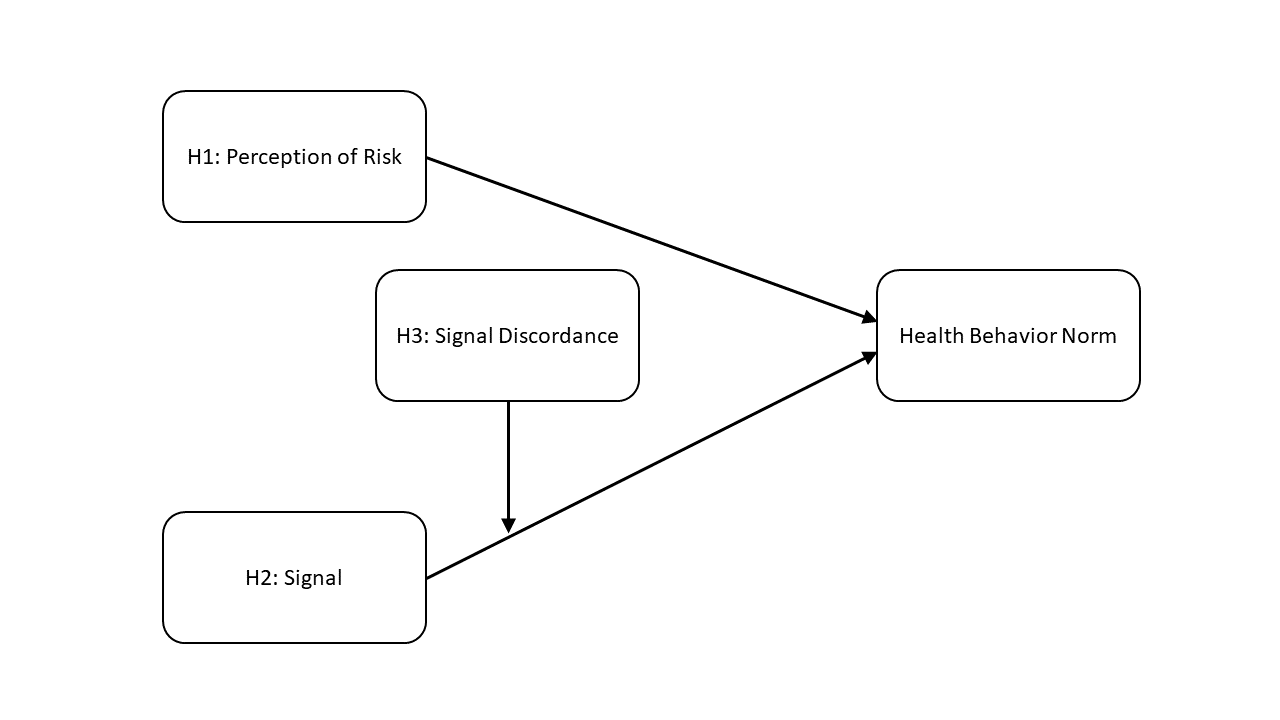
\includegraphics[width=0.8\linewidth]{figs/paper3/dag}}
\caption{Elaboratory Theoretical Model of Health Behavior Norms}\label{fig:dag}
\end{figure}

\hypertarget{associative-diffusion}{%
\subsection{Associative Diffusion}\label{associative-diffusion}}

While much of the social contagion literature, like the theories above, focuses
on structural boundaries and homophily as causes of how diffusion occurs,
\citet{goldbergSocialContagionAssociative2018} propose a
disrupting alternative mechanism. They argue that what actually diffuses during
social contagion are the perceptions about which beliefs or behaviors are
compatible with one another, what they call ``associative diffusion.'' This
argument that culture does not spread like a virus but instead is dependent on
how belief structures are connected to each other is important to test because
norms around health behaviors became politicized issues during the Covid-19
pandemic. This means that the stay-at-home or vaccination behavior themselves
were not contagious, but the cognitive association of precisely what social
distancing or vaccination uptake \emph{meant} were spreading between populations of
individuals. Moreover, as \citet{houghton20} outlines, diffusants - the things that are
diffusing through a population, are not independent of each other \citep{mason_etal07}. When we take into account the interdependence between different beliefs that are diffusing, such as Covid-19 is a hoax, social distancing saves
lives, the Covid-19 vaccine includes a microchip to control your thoughts, and lockdown
is against the rights guaranteed in the US constitution, we can imagine how
these various diffusants become associated together into structures of belief
through schemas of perception \citep{houghton20}. While this cognitive theory of cultural variation is difficult to test, the theory it supplies provides a solid framework for how behavioral norms formed during the pandemic.


The figure above illustrates how I interpret associative diffusion will impact
stay-at-home and vaccination rates in times of unsettled norms. An
individual enters this framework when they realize they don't have a normative
set of responses in their cultural toolkit to respond to an unfamiliar situation
they are presented with. Individuals look to norms to regulate behavior, avoid
deviance, and to maintain order \citep{horneNormsIntegratedFramework2020, shepherdStructurePerceptionHow2017}; when they don't have a normative behavior
to follow (or rebel against), individuals look to the other sources in their
``community'' to mimic behavior, such as high-status individuals, institutions,
and members of their social network. I theorize that individuals look towards
their physical community, to their social network, popular media (which may
include government and science recommendations), established norms that they may
find online through search, and to the real threat of infection (what would
happen if I do nothing about this norm). Following both the Integrated
Theoretical Framework of Norms \citep{horneNormsIntegratedFramework2020} and
associative diffusion \citep{dellapostaWhyLiberalsDrink2015, goldbergSocialContagionAssociative2018}, I theorize that individuals interpret
signals from their ``community'' through their cognitive biases and behavioral
predispositions to determine their formation of new behavioral norms.

There is some evidence I can draw upon to support the associative diffusion
fraemwork. For instance, there is a central conflict between religious and
scientific ideologies which I theorize leads more religious counties to reject
the stay-at-home order and vaccines \citep{evansReligionScienceEpistemological2008}
because the associative diffusion of these behaviors pits public health
recommendations against religious ideologies.
Furthermore, as COVID-19 has become a politically polarizing issue, conservative
ideology and a general mistrust of ``big government'' \citep{frank2007, gauchat2008} are likely to lead to resistance to the
government and scientific guidance.

\hypertarget{data-and-methods}{%
\section{Data and Methods}\label{data-and-methods}}

This article draws on two unique longitudinal datasets that I compiled for this
analysis from sources like Facebook, Google, CDC, and more. Because the
different datasets were on different scales (individual, zip-code, county,
state, designated market area) and time points (cross-sectional, longitudinal),
there was extensive data wrangling that had to be done to prepare these data for
statistical analysis. The steps taken to prepare each of the different model
features and where the data was sourced from is therefore covered in the
following sections before diving into modeling specifications.

\hypertarget{stay-at-home-rates}{%
\subsection{Stay at Home Rates}\label{stay-at-home-rates}}

\begin{table}[!ht]

\caption{\label{tab:google-desc-table}Descriptive Statistics for Stay-at-Home Models (county-level)}
\centering
\begin{tabular}{lrrrr}
\toprule
  & min & max & mean & sd\\
\midrule
Percent White & \num{0.14} & \num{0.98} & \num{0.81} & \num{0.15}\\
Percent College Graduates & \num{0.08} & \num{0.75} & \num{0.26} & \num{0.10}\\
Percent over 65 & \num{6.60} & \num{56.70} & \num{16.90} & \num{4.05}\\
Median Income & \num{28951.00} & \num{142299.00} & \num{59773.61} & \num{15264.50}\\
Monthly Unemployment Rate & \num{1.40} & \num{34.60} & \num{8.12} & \num{4.00}\\
Percent of GOP votes, 2016 & \num{0.08} & \num{0.90} & \num{0.57} & \num{0.15}\\
Percent Evangelical Christian & \num{0.00} & \num{0.67} & \num{0.20} & \num{0.14}\\
'Fox News' Trend & \num{0.00} & \num{204.08} & \num{29.59} & \num{16.94}\\
'Social Distancing' Trend & \num{0.00} & \num{500.00} & \num{20.64} & \num{25.36}\\
'Covid Conspiracy' Trend & \num{0.00} & \num{825.00} & \num{42.51} & \num{80.44}\\
Covid Case Rate & \num{0.00} & \num{343.71} & \num{21.17} & \num{27.44}\\
Week Number & \num{0.00} & \num{43.00} & \num{23.14} & \num{11.77}\\
Movement Signal & \num{-2.06} & \num{26.44} & \num{8.31} & \num{4.22}\\
Movement Discordance & \num{0.15} & \num{11.05} & \num{2.22} & \num{0.80}\\
\bottomrule
\multicolumn{5}{l}{\rule{0pt}{1em}Raw values presented in table. Values in models are normalized.}\\
\multicolumn{5}{l}{\rule{0pt}{1em}Notes: 1,375 counties, March 02 through December 28, 2020.}\\
\end{tabular}
\end{table}

\begin{figure}
{\centering 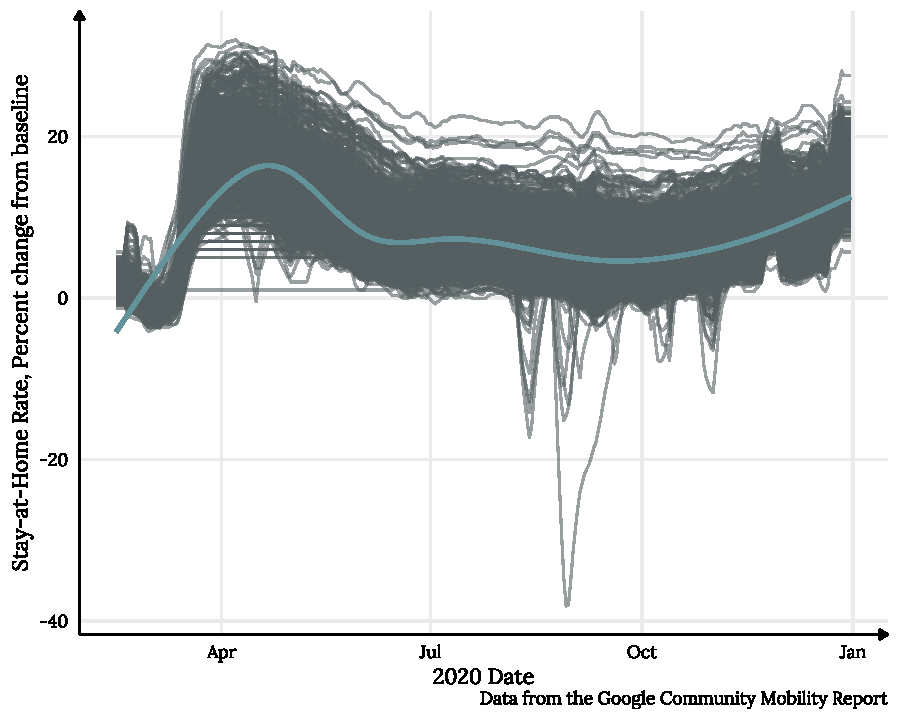
\includegraphics[width=0.8\linewidth]{figs/paper3/plot-google-1}}
\caption{Stay at Home Rates over Time}\label{fig:plot-google}
\end{figure}

My first dependent variable aims to operationalize behavioral norms as
stay-at-home rates with data from Google \citep{google2020}. While the Google
COVID-19 Community Mobility Reports include multiple measures of mobility based
on location and activity information, the change in time spent in residence
most closely aligns to an operationalization of an obedience to CDC and governor
orders, a new and emerging norm in 2020. The change in time spent in residence
variable represents percent change of time spent from Google Location History
within geographic areas that Google has designated as a residential area. These
data are aggregated to the county-level based on anonymized sets of data from
users who have turned on the Location History setting, which is off by default.
This means our sample is possibly skewed to people in the United States a) with
a mobile phone, b) with a Google account, and c) with knowledge of how to
synchronize their location history. Google has not made it clear whether there
are any weights in place to correct for these potential biases. Google
calculates the relative change in mobility in comparison to the median value of
movement in the area for the same the corresponding day of the week, during the
5-week period Jan 3--Feb 6, 2020. As Google did not provide data on certain US
counties if they did not have sufficient statistically significant levels of
data, my final county sample is \emph{n} = 1375
(compared to the total population of 3,107 US counties). Particular areas that
are excluded in this analysis include all counties in Alaska and DC, and over
half of the counties in North Dakota, South Dakota. A full list of excluded
counties available upon request. These data are longitudinal measures calculated
by creating a moving average of stay-at-home rates for each county (rolling
window width = 7 days) and then sampling every
Monday in the sample for 44 measures from March 02, 2020 through December 28,
2020.

\hypertarget{covid-vaccination-uptake}{%
\subsection{COVID vaccination uptake}\label{covid-vaccination-uptake}}

\begin{table}[!h]

\caption{\label{tab:vacc-desc-table}Descriptive Statistics for Vaccination Models (county-level)}
\centering
\begin{tabular}[t]{lrrrr}
\toprule
  & min & max & mean & sd\\
\midrule
Percent White & \num{0.08} & \num{1.00} & \num{0.83} & \num{0.17}\\
Percent College Graduates & \num{0.03} & \num{0.78} & \num{0.22} & \num{0.10}\\
Percent over 65 & \num{3.20} & \num{56.70} & \num{18.86} & \num{4.50}\\
Median Income & \num{21504.00} & \num{142299.00} & \num{53522.45} & \num{14312.25}\\
Monthly Unemployment Rate & \num{0.90} & \num{22.00} & \num{4.96} & \num{1.95}\\
Percent of GOP votes, 2020 & \num{0.09} & \num{0.94} & \num{0.64} & \num{0.16}\\
Percent Evangelical Christian & \num{0.00} & \num{1.31} & \num{0.22} & \num{0.16}\\
'Fox News' Trend & \num{5.00} & \num{405.88} & \num{72.12} & \num{27.38}\\
'Covid-19 vaccine' Trend & \num{0.00} & \num{755.56} & \num{74.67} & \num{70.33}\\
'Covid Conspiracy' Trend & \num{0.00} & \num{2000.00} & \num{56.05} & \num{189.61}\\
Covid Case Rate & \num{0.00} & \num{998.58} & \num{22.79} & \num{27.23}\\
Week Number & \num{1.00} & \num{35.00} & \num{18.00} & \num{10.10}\\
Vaccination Signal & \num{0.00} & \num{62.84} & \num{19.62} & \num{14.84}\\
Vaccination Discordance & \num{0.00} & \num{22.40} & \num{5.26} & \num{3.62}\\
\bottomrule
\multicolumn{5}{l}{\rule{0pt}{1em}Raw values presented in table. Values in Models are normalized.}\\
\multicolumn{5}{l}{\rule{0pt}{1em}Notes: 2,819 counties, January 04 through August 30, 2021.}\\
\end{tabular}
\end{table}

\begin{figure}
{\centering 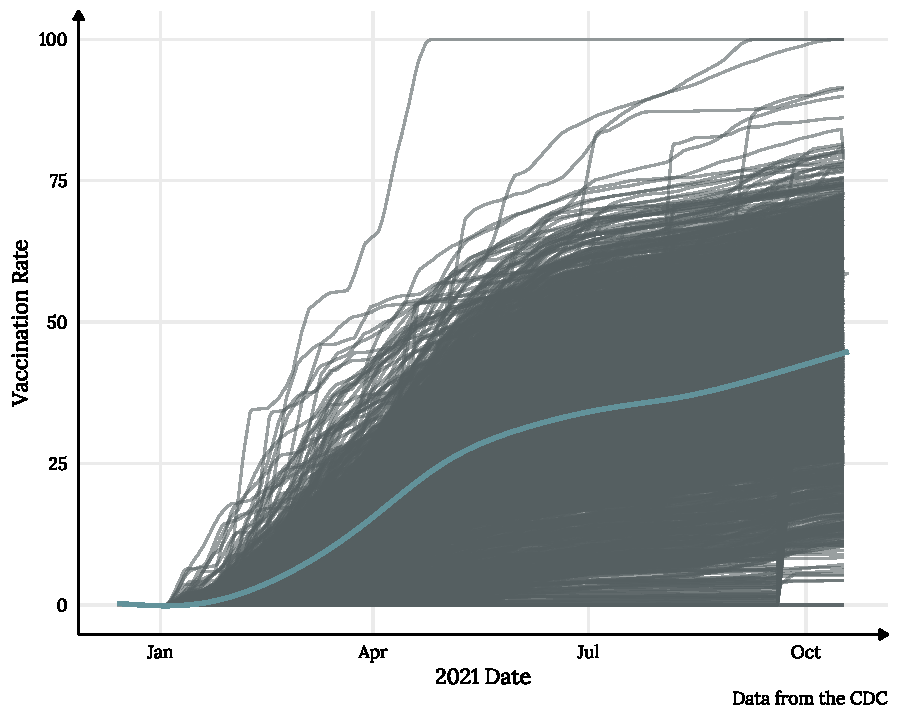
\includegraphics[width=0.8\linewidth]{figs/paper3/plot-vacc-1}}
\caption{Vaccination Rates over Time}\label{fig:plot-vacc}
\end{figure}

The second dependent variable aims to operationalize vaccination uptake through
vaccination rate information in the United States from January 2021 through
August 30 2021 \citep{cdcCOVID19Vaccination2021}. Data represents all vaccine partners including
jurisdictional partner clinics, retail pharmacies, long-term care facilities,
dialysis centers, Federal Emergency Management Agency and Health Resources and
Services Administration partner sites, and federal entity facilities.
Vaccination data is available for all US counties with the exception of parts of
California and Massachusetts, Hawaii, and Texas. In Texas and Hawaii, no county
level information is available, and California does not report the county of
residence for vaccinations when the county of residence has a population less
than 20,000 people. Finally, Massachusetts does not provide vaccination data for
Barnstable, Dukes, and Nantucket counties because of their small populations.
Therefore, my final county sample for vaccination rates is \emph{n} = 2819
(compared to the total population of 3,107 US counties). A list of included FIPS
are available upon request. Vaccination rates are scaled with a rolling mean
with a rolling window width of seven days to smooth out intra-week noise. I
sample every Monday between January 2021 through August 30, 2021 for 35 total
observations for each county.

\hypertarget{independent-variables-1}{%
\subsection{Independent Variables}\label{independent-variables-1}}

\hypertarget{network-signal}{%
\subsubsection{Network Signal}\label{network-signal}}

I utilize the likelihood of a friendship connection between counties
to create a county-level social network weighted by the probability of a tie.
Using this network and the two independent variables above, I examine how the
vaccination and stay-at-home rates of peer counties is contagious to the
ego-county. To do this, I first take the weighted average of each ego's network
signals using equation \eqref{eq:networksignal} where \texttt{x} denotes the
vaccination and stay-at-home rates of each alter county and \texttt{w} represents the
likelihood of a friendship connection between the ego county and each of their
alters, lagged by one week. This `signal' of norms gives us insight into the
coevolving contagion patterns of the new social norm being established. The
likelihood of friendship connection comes from the ``Social Connectedness Index''
\citep{Bailey2018, facebook20} which indexes the social links between geographies by
the likelihood of Facebook friends. It is an aggregated measure of Facebook
friendship connections between counties. It corresponds to ``the (relative)
probability that two arbitrary Facebook users across two geographies are friends
with each other.'' The data is available at various geographic aggregation
levels, such as U.S. zip codes or entire countries. However, data is only
available at one time point because Facebook has found that although there are
individual changes in friendship connections over time, the aggregate
statistical probabilities of friendship remain stable. This measure is based on
user-provided information and real-time location-service data gathered by
Facebook. Facebook data has been shown to be highly representative of the U.S.
population and Facebook friendship links largely represent real-world
friendships \citep{bailey_etal18, jones_etal13}. The data has been tested to show
how initial COVID-19 hotspots are related to subsequent virus spread to
non-hotspots, even after controlling for population density and geographic
distance \citep{Kuchler2020}.

\begin{equation}
signal = \frac{\sum_{i=1}^nw_ix_i}{\sum^n_{i=1}w_i} \label{eq:networksignal}
\end{equation}

\hypertarget{signal-discordance}{%
\subsubsection{Signal Discordance}\label{signal-discordance}}

The second independent variable, \emph{Signal Discordance}, builds on the network
signal but looks specifically at the extent to which a given ego-network
receives diverse contagion signals. Based on the hypothesis that when the
majority of alters is in concordance with each other, the signal to the ego is
reinforced and more impactful on the ego, a high discordance coefficient is
indicative of diverse signals which may prevent any clear interpretation of a
norm developing, whereas a low discordance coefficient would indicate reinforced
signaling. I use the formula to calculate weighted standard deviations, (see equation
\eqref{eq:signaldiscordance}) to provide a metric of a diversity of signals. In
this formula, \texttt{x} denotes the vaccination and stay-at-home rates of each alter
county and \texttt{w} represents the likelihood of a friendship connection between the
ego county and each of their alters, lagged by one week. Furthermore, \(\bar{x}^*\)
represents the weighted mean.

\begin{equation}
discordance = \sqrt{\frac{\sum_{i=1}^nw_i(x_i-\bar{x}^*)^2}{\sum^n_{i=1}w_i}} \label{eq:signaldiscordance}
\end{equation}

Figures \ref{fig:assortativity-vacc} and \ref{fig:discordancenetwork} provide
a visualization of both network signal and signal discordance for April 26, 2021
for 7 selected counties.\footnote{Figures in this paper were all created using ggplot2
\citep{wickham_etal, wickham11}, patchwork \citep{pedersen20}, and ggridges \citep{ggridges}}
While a county like Lake County, Ohio has low discordance meaning the signal of
vaccination rate is reinforced, Navajo County, Arizona receives very diverse
signals from their county-alters, negating any contagion effects. Figure
\ref{fig:discordancenetwork} explicitly outline how the weights and signals are
calculated for an ego with only 5 alters.

\begin{figure}
{\centering 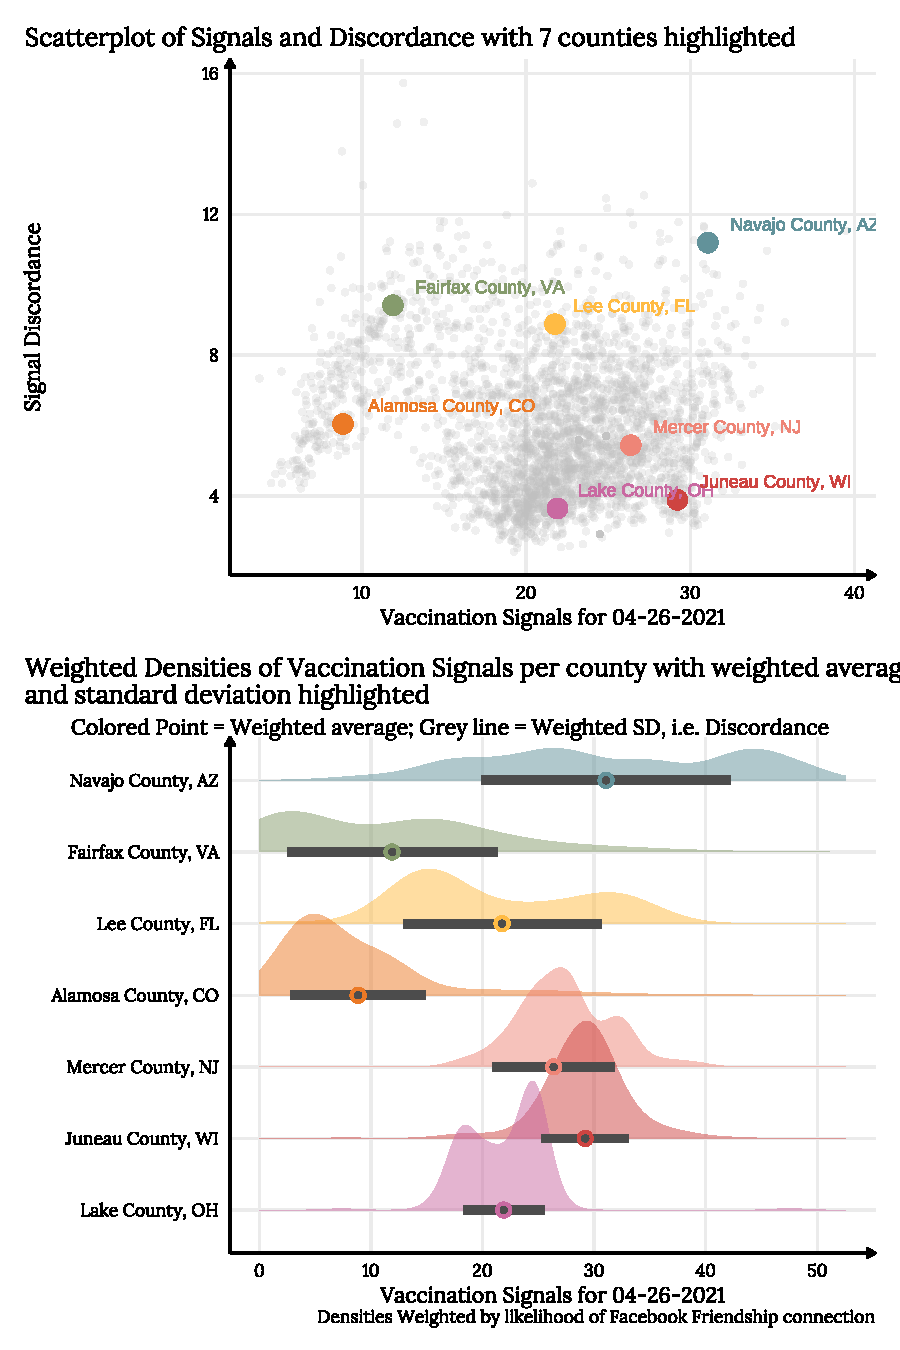
\includegraphics[width=0.7\linewidth]{figs/paper3/assortativity-vacc-1}}
\caption{How Signal Mean and Signal Assortativity are Measured}\label{fig:assortativity-vacc}
\end{figure}

\begin{figure}
\begin{center}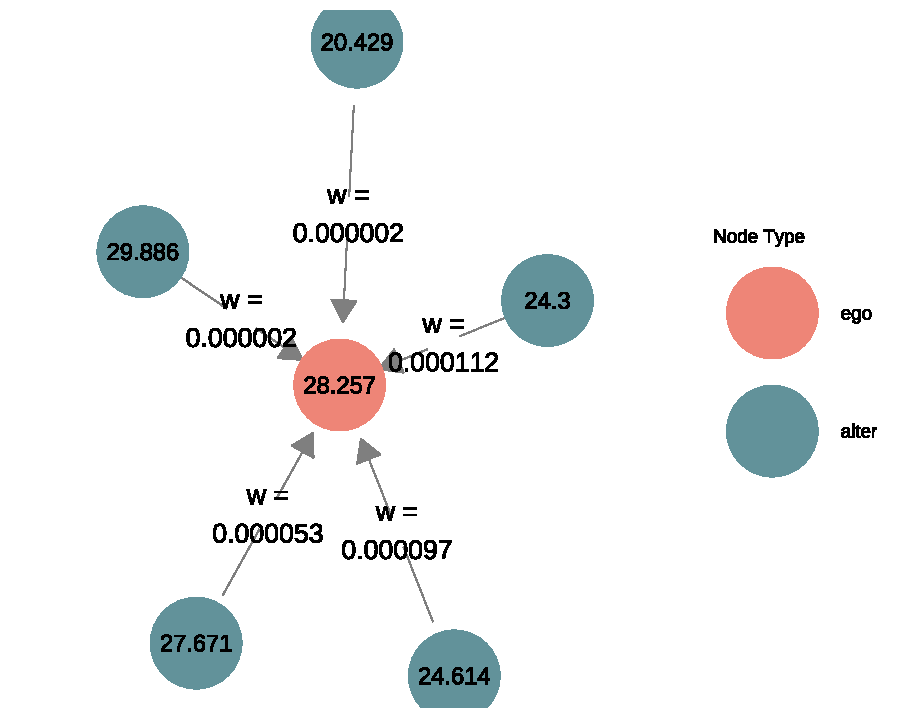
\includegraphics[width=0.5\linewidth,]{figs/paper3/discordancenetwork-1} 
  \begin{equation}
    w = \begin{bmatrix}0.0000015\\0.0000023\\0.0000527\\0.0000966\\0.0001119\end{bmatrix},  
    x = \begin{bmatrix}29.9\\20.4\\27.7\\24.6\\24.3\end{bmatrix} \longrightarrow
    \begin{matrix} \bar{x}, signal = 25.083\\ s, discordance = 1.41 \end{matrix} 
  \end{equation}
  \caption{Visualization of how Network Signal and Discordance are Calculated}
  \label{fig:discordancenetwork}
  \end{center}
\end{figure}

\hypertarget{covid-19-case-rates}{%
\subsubsection{Covid-19 Case Rates}\label{covid-19-case-rates}}

To estimate the concept of `real threat of infection' for a fear-based model of
health behaviors, the models use county-level Covid-19 case rates with
data compiled by The New York Times \citeyearpar{covid_data}. It is widely acknowledged that there are biases in this data due to inconsistencies and availability in testing as well as
different community propensity to test \citep{gu22, cdc20a}. However, it is the best
measure we have of actual case rates. County data are scaled with a rolling mean
with a rolling window width of seven days to smooth out intra-week noise. Case
Rate is measured as number of cases per 100,000 population. Observations vary
from a minimum of 0 to a maximum of 1,565 across the two datasets.

\hypertarget{online-norms}{%
\subsubsection{Online Norms}\label{online-norms}}

% TODO Mention that article-1 says that this can show interest (cite jungherr also) but does not show actions

To operationalize the search for online norms, I use Google search trends \citep{googletrends},
over the study period across individual designated media markets areas (DMAs), a
nonoverlapping aggregation of U.S. counties to 210 media markets based on
similar population clusters \citep{dma_key}. To investigate the rate of \emph{searching} for norms
online in both cases, I use the following search topics: `Social Distancing'
(2020, stay-at-home case only), `Covid-19 Vaccine' (2021, vaccination uptake case
only) and Covid Conspiracy (2020-2021, both cases). Search topics are a more
robust measurement than a single search term: topics are aggregations of the
rates of multiple, highly correlated search terms together into a cohesive
topic. For example, while `Beyoncé,' `Beyonce' and `beyonce knowles' are all
separate search terms, `Beyoncé Knowles' encompasses all of these into a single
search topic. While the data is originally on a scale of 0 to 100, with
100 being the maximum search popularity out of all DMAs, Google Search Trend are
now only available cross-sectionally (a single time period across a geography)
or time-series (a single geo-location across time). To remedy this and build a
longitudinal dataset of each search topic, I follow the method proposed in \citet[p. 5]{park_etal}.
This method involves building a dataset of unscaled
cross-sectional values, selecting a DMA to use to establish the rescaling ratio
(I use `Los Angeles CA'), and then finding the time-series values for the one
DMA. To find the rescaling ratio for each week in the time-series, you divide
the time-series value for each week by the cross-sectional value for each week,
resulting in a rescaling vector to be used for all weeks in the dataset across
geographies. To rescale each longitudinal value, multiply the respective week's
rescaling ratio by the cross-sectional value. Rescaled longitudinal data was
compared against time-series data for multiple test counties and was equivalent.
For a more in-depth explanation of this procedure, see \citet[p. 5]{park_etal}.

\hypertarget{pillars-of-convervatism}{%
\subsubsection{Pillars of Convervatism}\label{pillars-of-convervatism}}

Research has shown that stay-at-home rates and other pandemic health behaviors
are related to various `pillars of conservatism' \citep{gonzalez_etal21,hillBloodChristCompels2020,hillLoveThyAged2021, hillNastiestQuestion}. Namely, research shows that politically conservative
indicators, such as Republican political leadership, conservative Protestantism
and consumption of right-wing media are related to higher rates of movement and
lower rates of mask usage. Based on these findings, this article controls for
these factors in the following ways: to measure Republican political leadership,
I include percentage of votes for Donald Trump in the previous presidential
election; for the 2020 study, I use the 2016 results and for the 2021 study, I
use the 2020 results to infer proper time ordering. Second, to measure
conservative Protestantism, I employ the county's percentage of evangelical
Christians. These county-level data were collected through the 2010 U.S.
Religion Census: Religious Congregations and Membership Study \citep{grammich_etal18}. Finally, right-wing media consumption is assessed using
Google Search Trends to capture ``Fox News'' searches over the study period across
individual designated media markets areas (DMAs). I use this measure to indicate
active interest in and attention toward Fox News. Google Search Trends have been
validated for use in a range of research contexts and for use with survey data,
voting data, and ecological data \citep{bailPrestigeProximityPrejudice2019, reyesUsingInternetSearch2018, scheitleGoogleInsightsSearch2011, stephensdavidowitzCostRacialAnimus2014, swearingenGoogleInsightsSenate2014}.

\hypertarget{demographics}{%
\subsubsection{Demographics}\label{demographics}}

These models also control for (1) percent of the population that is above 65
years old (those most at risk of hospitalization), (2) percent of the population
that identifies as white, (3) percent of the population that holds a college
degree, (4) median income, and (5) monthly county unemployment rate. Measures 1
through 4 are obtained from the 2018 American Community Survey: 5-Year Estimates \citep{uscensusbureauAmericanCommunitySurvey2018}; unemployment rates are gathered
from the U.S. Bureau of Labor Statistics \citep{labor2020a}.

\hypertarget{analysis-and-results}{%
\section{Analysis and Results}\label{analysis-and-results}}

My analytic strategy proceeds in four steps. In Tables
\ref{tab:google-desc-table} (Stay-at-Home) and \ref{tab:vacc-desc-table}
(Vaccination Uptake), I present descriptive statistics for all study variables,
including variable ranges, means, and standard deviations across the two cases.
Then, in Tables \ref{tab:google-tab} - \ref{tab:vacc-tab}, I fit a series of
three linear mixed effects regression models using the nlme package in R
\citep{pinheiro_etal21, pinheiro_bates00} for our two cases, Stay-at-Home rates and
Vaccination rates. Linear mixed effects models are a form of hierarchical linear
models that contain both random and fixed effects. These models treat the
dependent variables as continuous. The following strategies I will outline are
identical for both case studies. Models 1 through 3 address hypotheses 1 through
3 respectively. Each model utilizes normalized independent variables, i.e.
variables that have been centered and scaled to have a mean of 0 and standard
deviation 1. The first model is a baseline linear mixed effects model that
employs all basic controls to predict the dependent variable, allowing both
time-varying and county-level variables to predict the outcome. All variables
have fixed effects, meaning that the county-level exogenous effects are
controlled for when estimating the coefficient. In addition, models are
specified with a random intercept per county. The lme models are set with a
autoregressive correlation structure (\texttt{correlation\ =\ corAR1()}) to control for
temporally autocorrelated error structures; models are also optimized using
Nelder--Mead, quasi-Newton and conjugate-gradient algorithms for box-constrained
optimization and simulated annealing (\texttt{control\ =\ lmeControl(opt\ =\ "optim")}).
This first model will address Hypothesis 1. To test hypothesis 2, I estimate
model 2 which builds on model 1 by first introducing vaccination signal. Because
the signal varies by week, I estimate this model with an interaction between
week and signal. And finally, because signal may have divergent effects across
counties, I set a random effect for signal nested by county. A visual
representation of this interaction can be seen in figures
\ref{fig:plot-google-h2} and \ref{fig:plot-vacc-h2}. Model 3 further
elaborates on the previous model by introducing both a fixed effect for signal
discordance and an interaction term between signal and discordance. Figures
\ref{fig:plot-google-h3} and \ref{fig:plot-vacc-h3} depict just how signal and
discordance interact across these two cases.

\hypertarget{stay-at-home-rate-results}{%
\subsection{Stay-at-Home Rate results}\label{stay-at-home-rate-results}}

\begin{table}[!h]

\caption{\label{tab:google-tab}Linear Mixed Effects Regression Results for Stay-At-Home Rates}
\centering
\fontsize{8}{10}\selectfont
\begin{tabular}[t]{lccc}
\toprule
  & Model 1 & Model 2 & Model 3\\
\midrule
Percent White & \num{0.088}*** & \num{0.058}** & \num{0.060}**\\
 & (\num{0.023}) & (\num{0.019}) & (\num{0.019})\\
Percent College Graduates & \num{-0.016} & \num{0.010} & \num{0.020}\\
 & (\num{0.028}) & (\num{0.023}) & (\num{0.024})\\
Percent over 65 & \num{-0.034}+ & \num{-0.031}* & \num{-0.037}*\\
 & (\num{0.018}) & (\num{0.015}) & (\num{0.015})\\
Median Income & \num{-0.042} & \num{-0.032} & \num{0.015}\\
 & (\num{0.030}) & (\num{0.024}) & (\num{0.025})\\
Monthly Unemployment Rate & \num{0.087}*** & \num{0.012}*** & \num{0.065}***\\
 & (\num{0.003}) & (\num{0.003}) & (\num{0.004})\\
Percent of GOP votes, 2016 & \num{0.077}* & \num{0.043} & \num{0.017}\\
 & (\num{0.032}) & (\num{0.026}) & (\num{0.027})\\
Percent Evangelical Christian & \num{-0.016} & \num{-0.008} & \num{-0.014}\\
 & (\num{0.022}) & (\num{0.018}) & (\num{0.019})\\
'Fox News' Trend & \num{-0.030}*** & \num{-0.028}*** & \num{-0.026}***\\
 & (\num{0.001}) & (\num{0.001}) & \vphantom{1} (\num{0.001})\\
'Social Distancing' Trend & \num{0.011}*** & \num{0.004}* & \num{0.001}\\
 & (\num{0.002}) & (\num{0.002}) & \vphantom{1} (\num{0.002})\\
'Covid Conspiracy' Trend & \num{0.024}*** & \num{0.006}*** & \num{0.010}***\\
 & (\num{0.002}) & (\num{0.002}) & (\num{0.002})\\
Covid Case Rate & \num{0.000} & \num{-0.009}* & \num{-0.007}+\\
 & (\num{0.004}) & (\num{0.004}) & (\num{0.004})\\
Week Number & \num{-0.002}+ & \num{-0.002}* & \num{-0.004}***\\
 & (\num{0.001}) & (\num{0.001}) & (\num{0.001})\\
Stay at Home Rate, county mean & \num{0.898}*** & \num{0.873}*** & \num{0.846}***\\
 & (\num{0.059}) & (\num{0.048}) & (\num{0.050})\\
Signal &  & \num{0.473}*** & \num{0.550}***\\
 &  & (\num{0.005}) & (\num{0.008})\\
Signal x Week &  & \num{-0.016}*** & \num{-0.018}***\\
 &  & (\num{0.000}) & (\num{0.000})\\
Signal Discordance &  &  & \num{-0.101}***\\
 &  &  & (\num{0.004})\\
Signal x Signal Discordance &  &  & \num{-0.092}***\\
 &  &  & (\num{0.002})\\
\midrule
Log.Lik. & \num{-23007.044} & \num{-19555.920} & \num{-18655.837}\\
\bottomrule
\multicolumn{4}{l}{\rule{0pt}{1em}N = 57,356, N of random Effects = 1375}\\
\multicolumn{4}{l}{\rule{0pt}{1em}* p $<$ .05. ** p $<$ .01. *** p $<$ .001 (two-tailed test).}\\
\multicolumn{4}{l}{\rule{0pt}{1em}Model 1 includes a random intercept for FIPS,}\\
\multicolumn{4}{l}{\rule{0pt}{1em}Models 2-3 include a random effect for Movement Signal by FIPS}\\
\end{tabular}
\end{table}


In Table \ref{tab:google-tab} and Figures \ref{fig:plot-google-h2} -
\ref{fig:plot-google-h3}, I present the elaboratory county-level models that
predict stay-at-home rates, or, time spent in residence. Model 1 addresses
hypothesis 1, that relatively higher local rates of infection will lead to
increased time spent in residence. This model's phi paramter is 0.933, which is
a good indicator that adjacent time points for each county are related and the
model is specified correctly (Finch, Bolin, and Kelley 2014). In this first model, many controls
have an impact on the outcome. For instance, when controlling for everything
else, the percent of GOP votes in 2016, the percentage of residents who identify
racially as White, and higher rates of unemployment increased the stay-at-home
rate while Searches for norms online seems to
have an effect on the outcome: searches for `Fox News' are associated with
decreased stay-at-home rates, while searching for both `Social Distancing' and
`Covid Conspiracy' tend to increase time spent in residence. Interestingly, the
perceived threat of the virus, measured through Covid-19 case rates, were not
significantly related to stay-at-home rates in model 1. In other words, for
every 1 standard deviation increase in Covid-19 case rates, stay-at-home rates
actually decreased by
0.0003 (\emph{p} = 0.936),
a very small and insignificant effect. In this case, I fail to reject the null
hypothesis that relatively higher local rates of infection will lead to
increased time spent in residence.

Table \ref{tab:google-tab} Model 2 investigates Hypothesis 2, that increased
average time spent in residence (signal direction) from alters will have a
positive effect on stay-at-home rates for the ego-county. This model builds on
model 1 by adding in the variable for Movement Signal (see \protect\hyperlink{network-signal}{Network
Signal} for specifications). For every one standard deviation
increase in the average time spent in residence of the county alters, an ego tends to also increase its' own stay-at-home rate by
0.473
(\emph{p} \textless{} 0.001). I am therefore able to reject my null hypothesis for hypothesis
2, that an increased average time spent in residence (signal direction) from
alters will have a positive effect on time spent in residence for the
ego-county.

\begin{figure}
{\centering 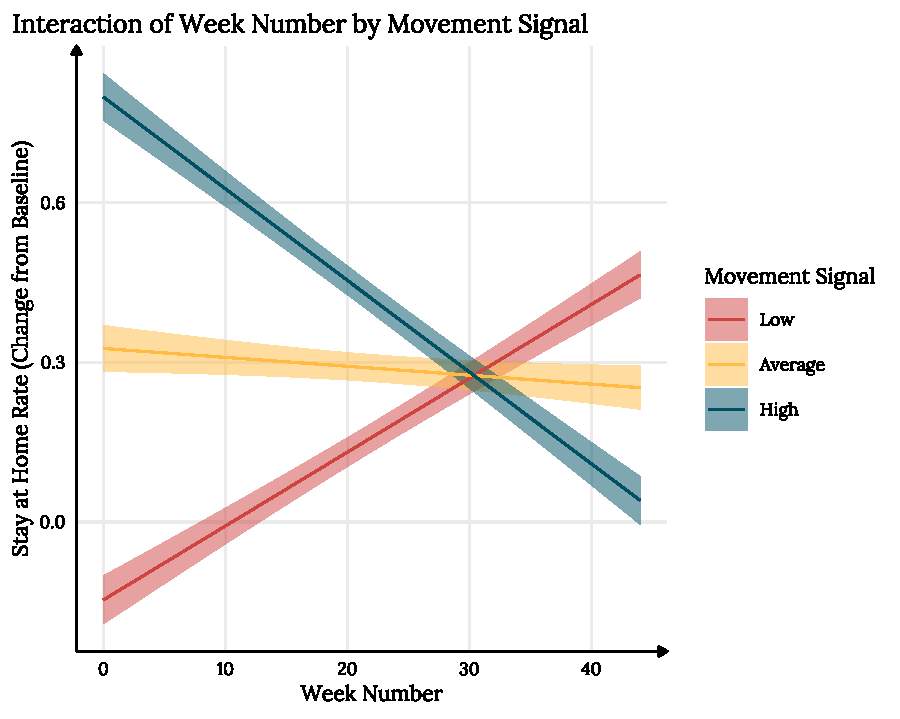
\includegraphics[width=0.8\linewidth]{figs/paper3/plot-google-h2-1}}
\caption{Predicted Values of Stay at Home Rate by Movement Signal}\label{fig:plot-google-h2}
\end{figure}

However, this coefficient is inadequate alone because the effect varies over
time; the interaction between week and movement signal is negative, meaning that
week partially moderates the effect of the signal. Figure
\ref{fig:plot-google-h2} illustrates this interaction. In the early days of the
Covid-19 pandemic, seeing a high rate of time spent in residence by alters led
to a high rate of staying-at-home for county egos. However, as the pandemic
progressed, these signals switched. In other words, towards the end of 2020,
other factors may have come into play and if a county saw its' alters social
distancing and spending time in residence, ego counties spent less time at home.
Theoretically, this may be because individuals saw their adjacent communities
with strong public health norms and felt safe and justified their own deviance.
However, if an ego county received signals that
others were failing to social distance, they were more likely to stay-at-home.
In this case, the threat of the virus may have been more evident for
individuals.

\begin{figure}
{\centering 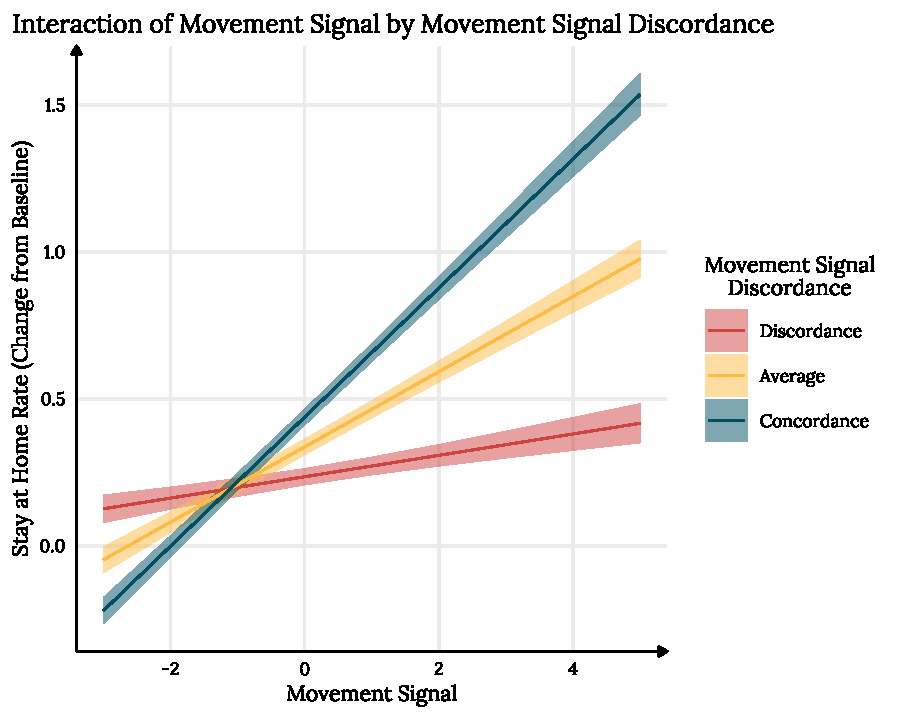
\includegraphics[width=0.8\linewidth]{figs/paper3/plot-google-h3-1}}
\caption{Predicted Values of Stay at Home Rate Moderated}\label{fig:plot-google-h3}
\end{figure}

Model 3 then adds the concept of Signal Discordance to investigate Hypothesis 3,
that the effect of signal direction on stay-at-home rates will be moderated by a
diversity in signals (\emph{discordance}). Many of the controls remain consistent
throughout the models, with the exception of `Social Distancing' Trend whose
effect has been completely mediated by the inclusion of signal discordance.
Importantly, signal discordance has a negative effect on stay-at-home rates,
where every one standard deviation increase in discordance lowers stay-at-home rates by
-0.101
(\emph{p} \textless{} 0.001). The interaction between signal and signal discordance have a
coefficient of a similar magnitude, with every one standard deviation increase
in discordance and signal resulting in
-0.092
lower rates of time spent in residence, indicating moderation. Figure
\ref{fig:plot-google-h3} illustrates the moderating effect that signal
discordance has on signal. Under high discordance, the social influence effect
is almost completely moderated because there is no clear story or norm forming.
However, under low discordance, the signal is condensed, allowing for social
influence to have an effect. Explicitly, if a county is receiving a wide array
of low and high signals, their stay at home rates won't be affected by social
contagion. When a signal is concentrated or in agreement, the theoretical effect
of movement signaling on the ego are the strongest. With this, I am able to
reject the null hypothesis of no relationship for hypothesis 3 and find that the
effect of signal direction on time spent in residence is moderated by diversity
in signals.

\hypertarget{vaccination-rate-results}{%
\subsection{Vaccination Rate results}\label{vaccination-rate-results}}

\begin{table}[!ht]

\caption{\label{tab:vacc-tab}Linear Mixed Effects Regression Results for Vaccination Rates}
\centering
\fontsize{8}{10}\selectfont
\begin{tabular}{lccc}
\toprule
  & Model 1 & Model 2 & Model 3\\
\midrule
Percent White & \num{0.023}+ & \num{-0.029}*** & \num{-0.027}***\\
 & (\num{0.012}) & (\num{0.003}) & (\num{0.003})\\
Percent College Graduates & \num{-0.004} & \num{0.009}* & \num{0.010}*\\
 & (\num{0.013}) & (\num{0.004}) & (\num{0.004})\\
Percent over 65 & \num{-0.012} & \num{-0.002} & \num{0.000}\\
 & (\num{0.008}) & (\num{0.002}) & (\num{0.002})\\
Median Income & \num{0.002} & \num{-0.017}*** & \num{-0.016}***\\
 & (\num{0.011}) & (\num{0.003}) & (\num{0.003})\\
Monthly Unemployment Rate & \num{-0.031}*** & \num{-0.014}*** & \num{-0.013}***\\
 & (\num{0.001}) & (\num{0.001}) & (\num{0.001})\\
Percent of GOP votes, 2020 & \num{-0.070}*** & \num{0.031}*** & \num{0.028}***\\
 & (\num{0.014}) & (\num{0.004}) & (\num{0.004})\\
Percent Evangelical Christian & \num{0.000} & \num{0.000} & \num{-0.001}\\
 & (\num{0.009}) & (\num{0.003}) & (\num{0.003})\\
'Fox News' Trend & \num{0.002}*** & \num{0.000} & \num{0.000}*\\
 & (\num{0.000}) & (\num{0.000}) & \vphantom{4} (\num{0.000})\\
'Vaccine' Trend & \num{-0.001}*** & \num{0.000} & \num{0.000}+\\
 & (\num{0.000}) & (\num{0.000}) & \vphantom{3} (\num{0.000})\\
'Covid Conspiracy' Trend & \num{0.000}* & \num{0.001}*** & \num{0.001}***\\
 & (\num{0.000}) & (\num{0.000}) & \vphantom{2} (\num{0.000})\\
Covid Case Rate & \num{-0.008}*** & \num{0.001}*** & \num{0.001}***\\
 & (\num{0.000}) & (\num{0.000}) & \vphantom{1} (\num{0.000})\\
Week Number & \num{0.067}*** & \num{0.011}*** & \num{0.011}***\\
 & (\num{0.000}) & (\num{0.000}) & (\num{0.000})\\
Vaccination Rate, county mean & \num{0.800}*** & \num{0.201}*** & \num{0.170}***\\
 & (\num{0.018}) & (\num{0.005}) & (\num{0.005})\\
Vaccination Signal &  & \num{0.854}*** & \num{0.865}***\\
 &  & (\num{0.005}) & (\num{0.006})\\
Vaccination Signal x Week &  & \num{-0.005}*** & \num{-0.003}***\\
 &  & (\num{0.000}) & (\num{0.000})\\
Vaccination Discordance &  &  & \num{-0.072}***\\
 &  &  & \vphantom{1} (\num{0.002})\\
Vaccination Signal x Discordance &  &  & \num{-0.051}***\\
 &  &  & (\num{0.002})\\
\midrule
Log.Lik. & \num{118677.013} & \num{160000.978} & \num{160638.703}\\
\bottomrule
\multicolumn{4}{l}{\rule{0pt}{1em}N = 99,890, N of random Effects = 2819}\\
\multicolumn{4}{l}{\rule{0pt}{1em}* p $<$ .05. ** p $<$ .01. *** p $<$ .001 (two-tailed test).}\\
\multicolumn{4}{l}{\rule{0pt}{1em}Model 1 includes a random intercept for FIPS,}\\
\multicolumn{4}{l}{\rule{0pt}{1em}Models 2-3 include a random effect for Movement Signal by FIPS}\\
\end{tabular}
\end{table}

In Table \ref{tab:vacc-tab} and Figures \ref{fig:plot-vacc-h2} -
\ref{fig:plot-vacc-h3}, I present the elaboratory county-level models that
predict vaccination uptake rates. The parameter phi in model 1 is .985, which is
a good indicator that adjacent time points for each county are related and this
is an appropriate modeling technique for the data \citep{finch_etal14}. Table
\ref{tab:vacc-tab} Model 1 addresses hypothesis 1, that relatively higher local
rates of infection will lead to increased vaccination uptake. In this first
model, we see various controls impacting vaccination rates. For instance, when
controlling for everything else, higher income areas lead to higher vaccination
uptake. On the other hand, counties with higher unemployment and higher votes
for Donald J. Trump in the 2020 election are associated with lower vaccination
rates. Interestingly, counties that search for Fox News are more likely to have
higher vaccination rates while those performing Google searches for information
about the vaccine are likely to have lower rates of vaccination. The test of
Hypothesis 1 also returns surprising results: every 1 standard deviation
increase in county Covid-19 case rates is expected to yield a -0.008 decrease in vaccination rates. This may be due to time ordering or reverse
causality, where individuals in counties who have higher rates of vaccination
are less likely to take tests to Covid-19 infections because of the higher
likelihood of asymptomaticity. However, it is important to note that the Case
Rate variable actually becomes distorted with the addition of Vaccination Signal
and Vaccination Discordance in models 2 and 3. Distortion occurs when the
direction of a focal relationship reverses sign once a third (distorter)
variable is controlled, in this case, those related to signal. Therefore, the
results of hypothesis 1 are quite inconclusive.

\begin{figure}
{\centering 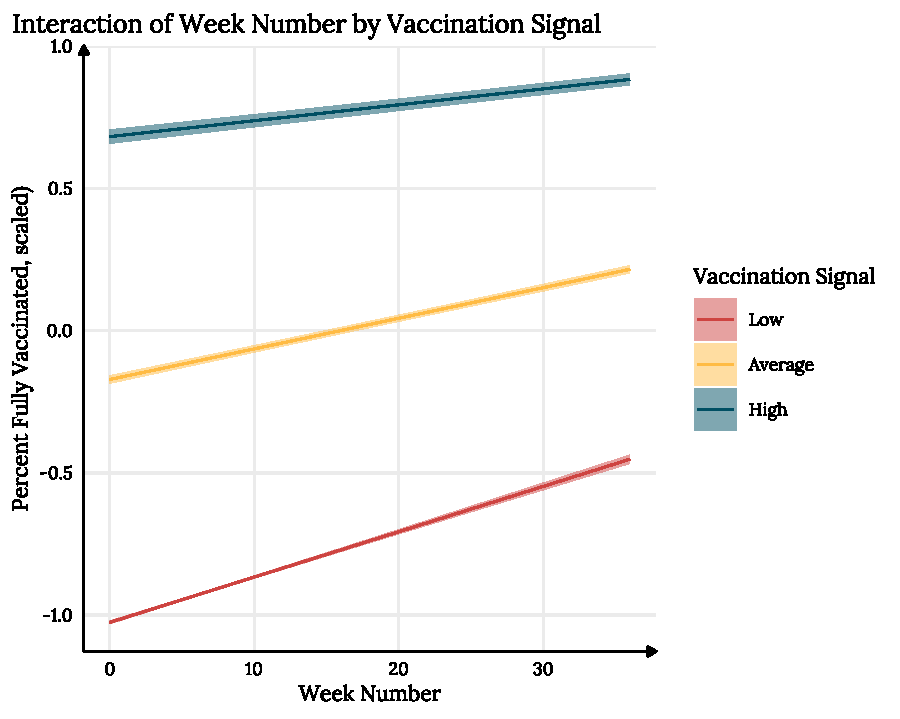
\includegraphics[width=0.8\linewidth]{figs/paper3/plot-vacc-h2-1}}
\caption{Predicted Values of Vaccination Rate}\label{fig:plot-vacc-h2}
\end{figure}

Table \ref{tab:vacc-tab} model 2 tests the hypothesis 2 that increase vaccine
uptake by alters will have a positive effect on vaccine uptake for the
ego-county. The results are incredibly clear: seeing alter counties receiving
vaccines is associated with higher vaccination rates. Specifically, a 1 standard
deviation increase in vaccine signal, the average rate of vaccination of a
county's alters, is associated with a
0.854
percent increase of vaccination rates for the ego county. The strength of this
result leads me to reject the null hypothesis for hypothesis 2 and find that
increased average time spent in residence (signal direction) from alters will
have a positive effect on time spent in residence for the ego-county. The
interaction of vaccine signal can be seen in Figure \ref{fig:plot-vacc-h2}.
While the interaction is not as extreme as the results for Hypothesis 2 for
Stay-at-Home rates, there is still a distinction between high and low
vaccination signals over time. The slope for Higher Vaccination Signal is less
pronounced than Low Vaccination Signal. This is likely an artifact where some
counties vaccinated broadly early on, so their vaccination rate stays rather
constant in later weeks. However, overall, the message is clear: ego-counties
who `see' high levels of vaccinations among their alters have higher vaccination
rates; those who don't see that social norm forming are much less likely to
vaccinate.

\begin{figure}
{\centering 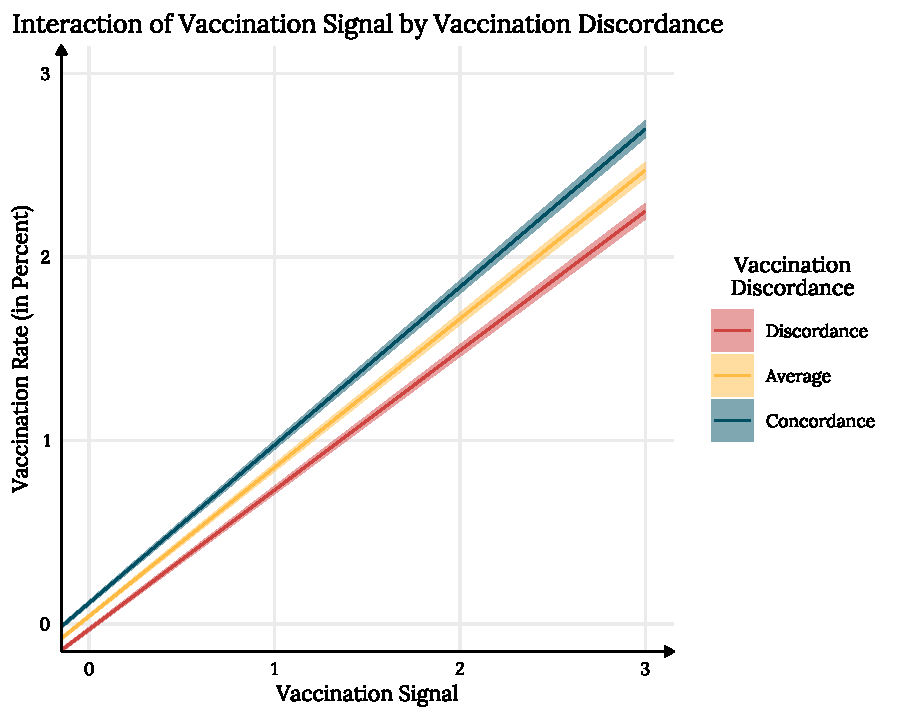
\includegraphics[width=0.8\linewidth]{figs/paper3/plot-vacc-h3-1}}
\caption{Predicted Values of Vaccination Rate}\label{fig:plot-vacc-h3}
\end{figure}

Table \ref{tab:vacc-tab} Model 3 then models the moderation of signal direction
for vaccine uptake by diversity in signals (\emph{Discordance}). This is a second
test of Hypothesis 3, that the effect of signal direction on vaccine uptake will
be moderated by diversity in signals. The coefficients in model 3 are largely
consistent with model 2 and there is very little change in the magnitude
or significance of the coefficients. Vaccination signal maintains to have a positive
effect on the alter's vaccination rates, while vaccination discordance has a negative effect on vaccination rates, where every one standard deviation increase in discordance lowers rates by -0.072 (\emph{p} \textless{} 0.001). The interaction between signal and signal discordance have a coefficient of a similar magnitude, with every one standard deviation increase
in discordance \emph{and} signal resulting in 
lower rates of vaccination. Figure \ref{fig:plot-vacc-h3} illustrates this
relationship, where there is slight moderation of the effect on vaccine signal
on vaccination rates. If a county receives consistently high signals, they are
more likely to have more residents vaccinated. If a county receives high but
inconsistent signals, they are still decently likely to raise vaccination rates
but to a lesser extent. While not as strong of moderation the the findings for
Stay-at-Home Rates for hypothesis 3, I also reject the null hypothesis and find
a moderation of the relationship between signal direction and vaccine uptake by
discordance.

\hypertarget{discussion-and-conclusion}{%
\section{Discussion and Conclusion}\label{discussion-and-conclusion}}

This paper examines how social norms are formed under conditions of uncertainty
using the case studies of stay-at-home rates and vaccination rates during the
Covid-19 pandemic. I test fear-based models of behavioral adaption to public
health recommendations as well as patterns of complex social contagion. This
article demonstrates that the establishment of social norms under patterns of
uncertainty in my two cases do follow the theorized framework of complex
contagion; however, I find a moderating effect of signal discordance to be an
overlooked factor in theories of contagion.

This study is sensitive to aggregation error and sampling error derived from the
multiple big-data sources \citep{facebook20, google2020}. The aggregation errors are
potentially linked to the assumption that the average stay-at-home behavior of a
county is a good representation of the diversity in behaviors within that
county. If stay-at-home rates are normally distributed, this is a correct
assumption to make; however, little is known about each county's underlying
distribution of behaviors that lead to the aggregate measures.

Regardless of limitations, this article is a unique and compelling contribution
to the academic study of social contagion and social norms. First, this article
demonstrates that it is possible to link, at least at a community level,
information search by individuals, social relationships, and observed health
behaviors without being limited to self-report measures of perceptions,
attitudes, or intentions about behavior. Sociological research has long debated
about the agency of individuals and the social and institutional structure in
which individuals are immersed. In this study, I aggregate beyond the individual
case to explore overall patterns of movement and vaccination which summarizes
individual agency of health behaviors together.

This article also provides a new adaption of the theory of complex contagion
using big data from the natural experiment of Covid-19. Because most studies of
complex contagion utilize agent-based modeling or studies of social media \citep{aralExerciseContagionGlobal2017,sprague_house17,bond_etal12,latane_etal94}, combining measures of actual behavioral outcomes with data from
social media websites provides a further test of ecological and external
validity for the theory.

Researchers of contagion and social networks should be interested in this study.
My theory of discordance, or a diversity of signals received, is not found in
the literature on complex contagion; complex contagion focuses on the number of
reinforcing actors, while other theories focus on how different diffusants
interact with each other \citep{houghton20,goldbergSocialContagionAssociative2018,mason_etal07}. Discordance, on the other hand, looks specifically at the context of the reinforcing actors among the other signals. This study finds that indeed the context of the signals matters for diffusion.